\documentclass[multi=page,12pt]{standalone}

\usepackage{graphicx}
\usepackage{psfrag}

\newcommand{\movedown}{\vphantom{\huge X}}
\begin{document}

\psfrag{x}[lt]{$x$}
\psfrag{F}{$F$}
\psfrag{L}{$L$}
\psfrag{EA}[l]{$EA$}
\psfrag{q}[B]{$q$}
\psfrag{k}{$k$}
\psfrag{n0}[lb]{$n_1$}
\psfrag{n1}[b]{$n_2$}
\psfrag{n2}[b]{$n_3$}
\psfrag{n3}[b]{$n_4$}
\psfrag{n4}[b]{$n_5$}
\psfrag{e0}[t]{$e_1$}
\psfrag{e1}[t]{$e_2$}
\psfrag{e2}[t]{$e_3$}
\psfrag{e3}[t]{$e_4$}

\begin{page}
\includegraphics[scale=0.8]{barDefinition0}
\end{page}

\begin{page}
\includegraphics[scale=0.8]{barDefinition1}
\end{page}

\begin{page}
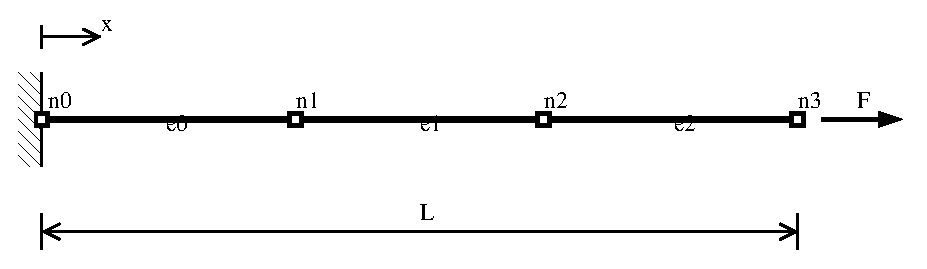
\includegraphics[scale=0.8]{barDefinition2}
\end{page}


\begin{page}
\psfrag{n0}[lt]{\movedown$n_1$}
\psfrag{n1}[t]{\movedown$n_2$}
\psfrag{n2}[t]{\movedown$n_3$}
\psfrag{n3}[t]{\movedown$n_4$}
\psfrag{n4}[t]{\movedown$n_5$}
\includegraphics[scale=0.8]{barDefinition3}
\end{page}

\end{document}
